\subsection*{A6.5}
\subsubsection*{(a)}
\paragraph{}
From the derivative constraint, we must have
\begin{align*}
\frac{y_{i+1}-y_i}{\beta} \leq z_{i+1} - z_i \leq \frac{y_{i+1}-y_i}{\alpha}, \qquad i =1,...,m-1 
\end{align*}
\paragraph{}
Therefore we can solve the following function
\begin{align*}
&\text{minimize}\qquad \sum_{i=1}^{m}||z_i - a_i^Tx||_2 \\
&\text{subject to}\qquad \frac{y_{i+1}-y_i}{\beta} \leq z_{i+1} - z_i \leq \frac{y_{i+1}-y_i}{\alpha}, \qquad i =1,...,m-1, 
\end{align*}
\paragraph{}
with variable $z \in R^m,\ x \in R^n$.
\subsubsection*{(b)} 
\verbatiminput{main.m}
\begin{figure}
	\centering
	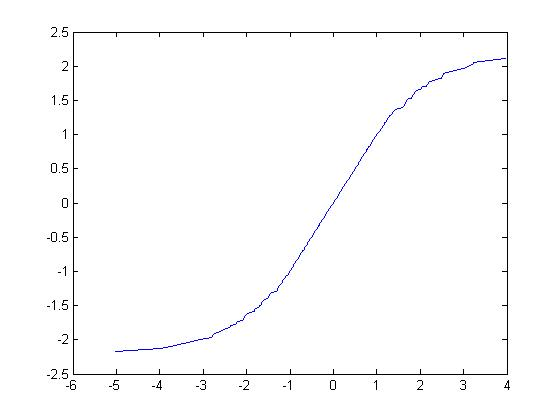
\includegraphics[scale=0.5]{z}
	\caption{Estimation of $\phi(z)$}
\end{figure}
\begin{figure}
	\centering
	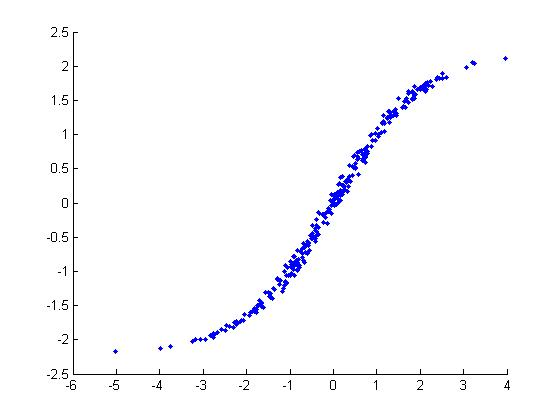
\includegraphics[scale=0.5]{x}
	\caption{Estimation of $a_i^Tx$}
\end{figure}
